\chapter{Modelo de maturidade}


	Um modelo de maturidade serve para avaliar a aptidão de uma organização afim de gerenciar seus projetos, são avaliados de acordo com as boas práticas de gerenciamento entre outros. Existem dois modelos de maturidade bastante utilizados pelas empresas brasileiras: o CMMI e o MPS.BR.

	O CMMI é um modelo de maturidade para desenvolvimento de software criado pelo SEI. Esse modelo é definido em áreas de processos que está vinculado às práticas relacionada satisfazendo um conjunto de objetivos oferecendo duas formas de abordagem diferentes para a melhoria de processos: modelo em estágio e modelo contínuo.
	
	O MPS é um programa para Melhoria de Processo do Software Brasileiro coordenado pela SOFTEX, com suporte do Ministério da Ciência e da Tecnologia, da FINEP e do BID. O MPS.BR é estruturado nos conceitos de maturidade dos processos para avaliação e melhoria da qualidade dos produtos de software e afins.

	\begin{figure}[!htpb]
			\centering
			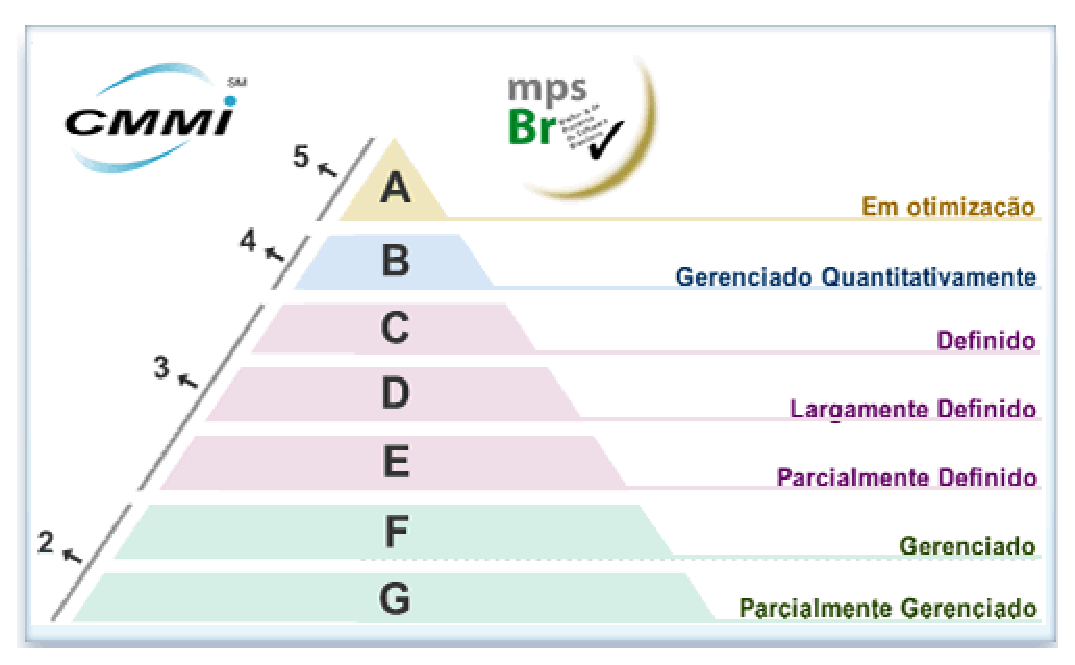
\includegraphics[scale=0.5]{figuras/maturidade/cmmi_mps}
			\caption{Níveis de maturidade}
	\end{figure}

	Nas seções a seguir será apresentados os resultados esperados na perspectiva de gerência de requisitos e de desenvolvimento de requisitos de acordo com o MPS.BR atrelado com o processo de Engenharia de Requisitos desenvolvido neste projeto.

	\section{Gerência de requisitos}

	O objetivo da gerência de requisitos é controlar a evolução dos requisitos, seja por constatação de incosistência entre os requisitos registrados até o momento (Hazan).

	\subsection{Resultados Esperados: GRE01}

	Neste nível é esperado que o entendimentos dos requisitos seja obtido junto com ao cliente. As atividades contidas no processo atreladas a este resultado são: Definir temas estratégicos, definir épicos, definir {\itshape epic enablers}, priorizar épicos, definir {\itshape features}, definit {\itshape feature enablers}. Todas estas atividades estão atreladas ao entendimento de requisitos no cliente, presente na fase inicial do modelo do processo, algumas destas atividades estão contidas em nível de portifólio, outras em nível de programa.

	\subsection{Resultados Esperados: GRE02}

	Neste nível os requisitos são avaliados utilizando critérios objetivos e o comprometimento da equipe e com isso é obtido um comprometimento da equipe. A atividade de planejar {\itshape PI} faz parte deste resultado esperado pois é neste estágio do processo que se espera a definição de datas, quantidade de interações prevista para a {\itshape features} e definição de documento de visão.


	\subsection{Resultados Esperados: GRE03}

	Neste nível é esperado que seja mantida e estabelecida a rastreabilidade bidirecional entre os requisitos e os produtos de trabalho. As atividades contidas no processo relacionadas a este resultados são as atividades relacionadas ao levantamento de requisitos: definir temas estratégicos, definir épicos, denir {\itshape epic enablers} e {\itshape feature enablers}, priorizar épicos e planejar {\itshape PI} pois é aonde define a rastreabilidade de acordo com os artefatos presentes nesta atividade.

	\subsection{Resultados Esperados: GRE04}
	
	É esperado neste estágio que revisões em planos e produtos de trabalho do projeto sejam realizadas com o intuito de identificar e corrigir as inconsistências em relação aos requisitos. Atividades do processo que está intimamente ligda a este resultado é realizar a restropectiva da iteração e realizar revisão da iteração.

	\subsection{Resultados Esperados: GRE05}

	Neste nível é esperado que mudanças nos requisitos sejam gerenciadas ao longo do projeto. Existem várias atividades que ocorrem em paralelo a outroscontidas no processo que está relacionada este resultado como: Gerenciar mudanças de requisitos na iteração, gerenciar mudanças de requisitos a nível de portifólio e gerenciar mudança de requisitos a nível de programa.

	\section{Desenvolvimento de Requisitos}

		O objetivo do desenvolvimento de requisitos é em geral definir os requisitos do cliente de tal maneira que esteja atrelado o produto e os componentes do mesmo.

	\subsection{Resultados Esperados: DRE01}
	Neste nível é esperado que as necessidades, expectativas e restrições do cliente, tanto do produto como quanto de suas interfaces sejam identificadas. As atividades contidas no processo ligadas a este resultado são: definir temas estratégicos, definir épicos, definir {\itshape epic enablers}, priorizar épicos, definir features e definir {\itshape features enablers}, são atividades que estão na fase inicial de compreensão da necessidade do cliente.

	\subsection{Resultados Esperados: DRE02}
	É esperado neste nível que um conjunto definido de requisitos do cliente seja especificado e priorizado a partir das necessidades expectativa e restrições identificadas. Priorizar épicos, priorizar features e planejar {\itshape PI} são atividades que fazem parte deste resultado esperado, no caso do planejamento do {\itshape PI} é a fase final das prioridades e aonda as features serão definidas para o dessenvolvimento.

	\subsection{Resultados Esperados: DRE03}
	Neste estágio é esperado que seja definido a partir dos requisitos do cliente um conjunto de requisitos funcionais e não funcionais do produto e dos componentes do produtos que descrevem a solução do problema a ser resolvido. Atividades atreladas a este resultado: definir {\itshape epic enbalers} e definir {\itshape feature enablers} atividades que representam requisitos funcionais e adicionando os requisitos não funcionais.

	\subsection{Resultados Esperados: DRE04}
	Neste nível é esperado que os requisitos funcionais e não funcionais de cada componente do produto sejam refinados, elaborados e alocados. A atividaade atrelada a este resultado e o planejamento do {\itshape} PI, pos é a atividade final aonde os epicos e a {\itshape features} estarão bem definidas por prioridade e que futuramente serão quebradas em tarefas a nível de desenvolvimento.

	\subsection{Resultados Esperados: DRE05}
	É espearado nese nível que sejam definidas interfaces internas e externas ao produto e de cada componente do produto. As atividades presentes no processo que podem ser vinculadas a este resultado são: definir features e definir {\itshape epic enablers} aonde são tomadas decisões de características do projeto. 

	\subsection{Resultados Esperados: DRE06}
	Neste estágio é esperado que sejam desenvolvidos os conceitos operacionais e cenários. As atividades relacionadas a este resultado são: planejar {\itshape} PI, desmembrar features em user stories e priorizar user histories, pois é aonde que irão descrever cenários a nível de usário de particularidades do projeto.

	\subsection{Resultados Esperados: DRE07}
	Neste nível é esperado que os requisitos sejam analisados, usando critérios definidos, para balancear as necesisdades dos interessados com as restrições identficadas. Priorizar épicos, features e planejar {\itshape PI} são tarefas ligadas a este resultado uma vez que é definida a prioridade das necessidades do cliente e é definido o processo a nível de time.

	\subsection{Resultados Esperados: DRE08}
		E finalmente é esperado aqui que os requisitos sejam validados. As atividades relacionadas a este resultado são: realizar revisão da iteração e realizar restropectiva da iteração aonde a nível de time as features são validadas na perpectiva da metodoligia ágil em conjunto com o stakeholders presentes no projeto.

